
Quaternions offer a reliable means of representing rotations in 3-dimensional space. The calculations required to manipulate them are more computationally efficient than matrix operations. Quaternions also do not suffer from the potential ambiguity inherent in representing rotations with 3-dimensional vectors storing values for pitch, roll, and yaw. Pitch, roll, and yaw (rotations in the transverse axis, longitudinal axis, and normal axis, respectively) are visualized in Figure \ref{fig:pitch_roll_yaw}, from \cite{pitch_roll_yaw_dji_source}. These 3-dimensional vectors suffer from loss of information if 2 of the rotational axes become aligned (gimbal lock), and from not providing a single, unique representation for each possible normalized rotation. For these reasons, quaternions are the default data object used to describe rotations in robotics and avionics. A detailed mathematical examination of quaternions is beyond the scope of this project. However, the main ideas behind using quaternions to represent rotation are that they can efficiently be composed with one another, and they represent rotation unambiguously. Mathematically rigorous definitions and explanations of the operations that are relevant to quaternions, as well as the history therein, can be found in \cite{quaternions_reference}.

\begin{figure}
    \centering
    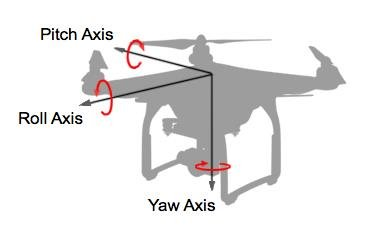
\includegraphics[width=0.35\textwidth]{images/pitch_roll_yaw_dji.png}
    \caption{Visualization of pitch, roll, and yaw.}
    \label{fig:pitch_roll_yaw}
\end{figure}

% Quaternions, as the name suggests, are made up of 4 components. A quaternion $q_1$ is defined in Equation \ref{equation:q_1}:
%     \begin{equation}
%         q_1 = w_1 + x_1i + y_1j + z_2k
%         \label{equation:q_1}
%     \end{equation}
% where $w_1,x_1,y_1,z_1 \in \mathbb{R}$ and $i,j,k$ are orthogonal unit vectors representing typical rotational axes $x,y,z$.  satisfying Equation \ref{equation:quaternion_complex_numbers}.
%     \begin{equation}
%         i^2 = j^2 = k^2 = ijk = -1
%         \label{equation:quaternion_complex_numbers}
%     \end{equation}

% \noindent
% {\color{red} The scalars $x_1,y_1,z_1$ represent the magnitudes of the angles of rotation $\theta_x, \theta_y, \theta_z$ about the axes $x,y,z$ respectively. } Let $\theta$ represent the rotation of $q_1$ about its axis defined by $x_1,y_1,z_1$, then $w$ is defined as in Equation \ref{equation:quaternion_w}:
% \begin{equation}
%     w = \cos \left( {\frac{\theta}{2}} \right)
%     \label{equation:quaternion_w}
% \end{equation}

% \noindent
% Let a second quaternion $q_2$ is defined as in Equation \ref{equation:q2}, again with $w,x,y,z \in \mathbb{R}$, and $i,j,k$ represent the same values as in Equation \ref{equation:q_1}:
% \begin{equation}
%     q_2 = w_2 + x_2i + y_2j + z_2k
%     \label{equation:q2}
% \end{equation}

% \noindent
% Then, in order to ``add'' the rotation described by $q_2$ to the rotation described by $q_1$, the quaternions are \textit{multiplied} using the Hamilton product, as in Equation \ref{equation:quaternion_multiplication}:
% \begin{equation}
%     q_3 = \left( w_2 + x_2i + y_2j + z_2k \right) \left( w_1 + x_1i + y_1j + z_2k \right)
%     \label{equation:quaternion_multiplication}
% \end{equation}

% \noindent
% The resulting quaternion $q_3$ is then equivalent to rotating by $q_1$ and then by $q_2$. In order to ``subtract'' rotations, the inverse of a quaternion is with respect to the Hamilton product is used, as in equation \ref{equation:quaternion_inverse}:
% \begin{equation}
%     q_2^{-1} = \dfrac{1}{w_2^2 + x_2^2 + y_2^2 + z_2^2}\left(w_2 - x_2i - y_2j - z_2k\right)
%     \label{equation:quaternion_inverse}
% \end{equation}

% \noindent
% The result of rotating first by $q_1$ and then by the inverse of $q_2$ can be found by taking the Hamilton product of $q_1$ and $q_2^{-1}$, similarly to Equation \ref{equation:quaternion_multiplication}.

The Transform 2 library (\texttt{tf2}) provides implementations of these data structures and the relevant operations within the ROS infrastructure. The Geometry Messages library (\texttt{geometry\_msgs}) provides message definitions for efficiently representing quaternions in message passing. This project employs these libraries instead of re-inventing the wheel in this area.